\begin{tutorial}{Рецепт пельменей}

По условию задачи нам нужно уметь находить первый минимум на отрезке от $1$ до $x$ и последний минимум на отрезке от $x$ до $n$, и затем увеличивать найденный элемент на $1$. Это стандартная задача \textit{RMQ (Range minimum query)}. Ограничения позволяют решать эту задачу за время $O(n~log~n)$ с использованием, например, \textit{дерева отрезков}.

Но данная задача имеет также линейное решение (за $O(n)$). Так как мы находим \textbf{первый} минимум на \textbf{префиксе} и \textbf{последний} минимум на \textbf{суффиксе}, то наш массив всегда имеет следующий вид:
\begin{itemize}
  \item слева~--- невозрастающий префикс (возможно нулевой длины);
  \item справа~--- неубывающий суффикс (возможно нулевой длины);
  \item между ними~--- подотрезок ненулевой длины, состоящий из одинаковых минимальных элементов массива. Далее будем называть его \textit{дном(bottom)}. $bottom_l$~--- индекс левого края дна, $bottom_r$~--- индекс правого края дна.
\end{itemize}

\begin{center}
  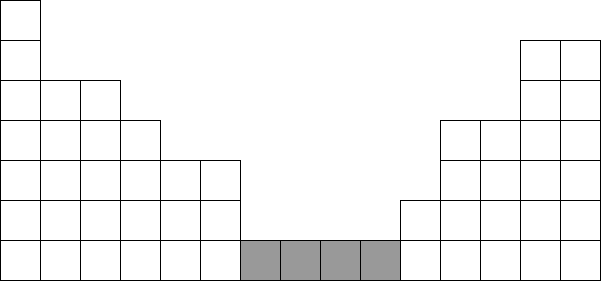
\includegraphics [width=.95\textwidth] {1.png}

  \textit{Для массива $[7, 5, 5, 4, 3, 3, 1, 1, 1, 1, 2, 4, 4, 6]$. Серым обозначено дно}
\end{center}

Обозначим массив как $a$. При запросе \texttt{x l}:
\begin{itemize}
  \item Если $x \ge bottom_l$, то увеличивается элемент $a[bottom_l]$, а $bottom_l$ увеличивается на $1$;
  \item Если $x < bottom_l$, то увеличивается самый левый элемент, равный $a[x]$ в~подотрезке из элементов $a[x]$ в невозрастающем префиксе. В нём подотрезок из элементов $a[x]$ укорачивается слева, а подотрезок из элементов $a[x] + 1$ увеличивается справа.
\end{itemize}

Аналогично при запросе \texttt{x r}:
\begin{itemize}
  \item Если $x \le bottom_r$, то увеличивается элемент $a[bottom_r]$, а $bottom_r$ уменьшается на $1$;
  \item Если $x > bottom_r$, то увеличивается самый правый элемент, равный $a[x]$ в~подотрезке из элементов $a[x]$ в невозрастающем суффиксе. В~нём подотрезок из элементов $a[x]$ укорачивается справа, а подотрезок из элементов $a[x] + 1$ увеличивается слева.
\end{itemize}

\begin{center}
  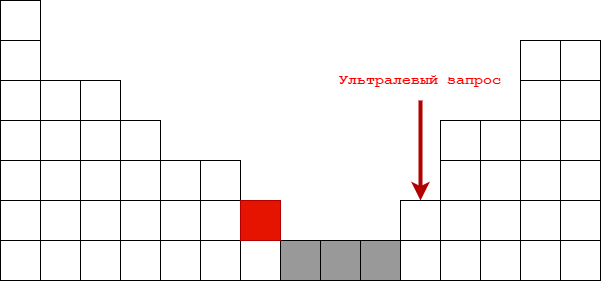
\includegraphics [width=.95\textwidth] {2.png}

  \textit{После запроса \texttt{11 l}}
\end{center}

\begin{center}
  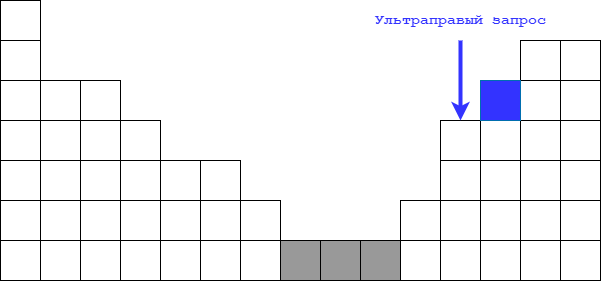
\includegraphics [width=.95\textwidth] {3.png}

  \textit{После запроса \texttt{12 r}}
\end{center}


\begin{center}
  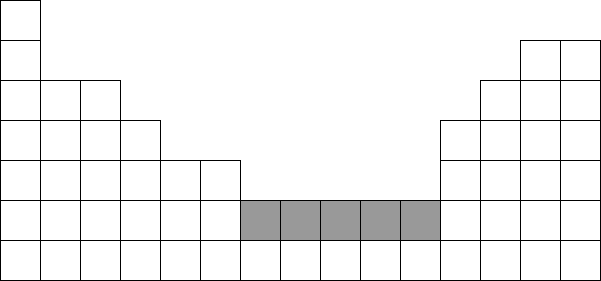
\includegraphics [width=.95\textwidth] {4.png}

  \textit{Новое дно после трех запросов \texttt{8 r}}
\end{center}

Промоделируем задачу. Будем поддерживать правую и левую границы подотрезков равных элементов в невозрастающем префиксе и неубывающем суффиксе. При увеличении элемента $a[x]$ соответствующая граница подотрезка с элементами $a[x]$ уменьшается, а соответствующая граница подотрезка с элементами $a[x] + 1$ увеличивается. Когда подотрезки сольются, обновляем дно.

\end{tutorial}
